\section{Durchführung}

\begin{figure}[tb]
  \centering
  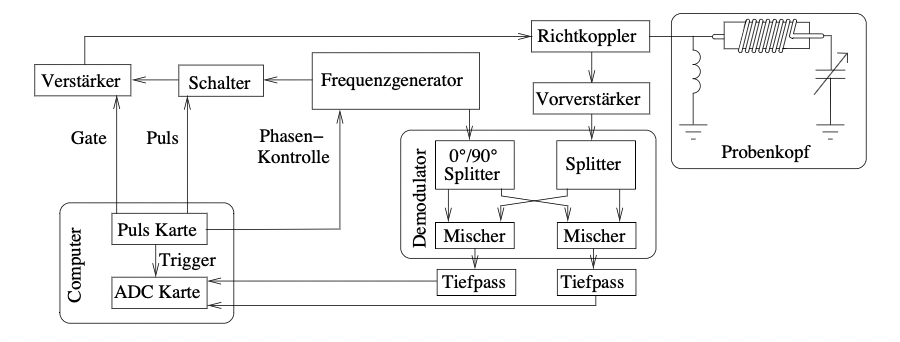
\includegraphics[width=\textwidth,keepaspectratio]{schaltbild.png}
  \caption{Blockschaltbild der verwendeten Messapparatur\cite{info}.}
  \label{fig:schaltbild}
\end{figure}

Ein Blockschaltbild der verwendeten Apparatur ist \autoref{fig:schaltbild} zu entnehmen. Diese ist bereits richtig verkabelt und muss vor den ersten Messungen nur noch justiert werden.

\subsection{Justage}
Zur Justage wird zunächst die Larmorfrequenz eingestellt. Diese lässt sich daran erkennen, dass der FID keine Schwingungen enthält.
Zur Messung der Induktion wird Quadraturdetektion genutzt. Hierbei wird das Signal $S$ mit einer Spannung mit der Larmorfrequenz überlagert bzw. heruntergemischt. Dieses Signal wird als $S_X$ bezeichnet. Dadurch sind die Phase und die Differenzfrequenz zwischen Signal und Referenzspannung messbar. Da hierbei die Information über die Größe des Signalbeitrags vor dem Mischen verloren geht, wird das Signal zudem mit der um $\SI{90}{\degree}$ verschobenen Referenzspannung heruntergemischt. So wird das Signal $S_y$ erhalten. Das Ergebnis ist als Wechsel in das rotierende Koordinatensystem zu verstehen, es gilt also $S(t) = S_x + i S_y \sim M(t) = M_x + i M_y$. Die Quadraturdetektion wird so eingestellt, dass ein möglichst großer Anteil des Signals im Realteil ist.
Weiterhin muss das Magnetfeld so eingestellt werden, dass die Feldhomogenität maximal ist. Dies ist daran zu erkennen, dass der FID eine möglichst hohe Abklingzeit hat, da in diesem Fall Diffusionseffekte einen minimalen Beitrag liefern.
Außerdem müssen die benötigte Zeitspanne für den $\SI{90}{\degree}$- und den $\SI{180}{\degree}$-Puls bestimmt werden.
Im Anschluss ist alles justiert und die Messungen können begonnen werden. Um eine veränderte Temperatur im Verlauf der Messungen möglichst als Fehlerquelle auszuschließen wird vor jeder Messreihe die Temperatur in der Messapparatur gemessen.

\subsection{Messungen zur Bestimmung der Relaxationszeiten und Diffusionskonstanten}

Zur Bestimmung von $T_1$ wird die \textit{Inversion Recovery} genutzt. Hierbei wird die Magnetisierung in $z$-Richtung unter Variation der Zeit $t$ zwischen Inversion und Drehung in die $x$-$y$-Ebene variiert. Es werden $21$ Messwerte im Bereich von $\SI{e-4}{\second}$ bis $\SI{10}{\second}$ aufgenommen, wobei die Abstände zwischen den Messwerten auf eine logarithmische Skala angepasst sind.

Die Bestimmung von $T_2$ geschieht mittels Meiboom-Gill-Methode. Hierbei werden nach dem $\SI{90}{\degree}$-Puls $100$ um $\SI{90}{\degree}$ phasenverschobene $\SI{180}{\degree}$-Pulse eingestrahlt und $\tau$ wird so eingestellt, dass die Amplitude des 100. Echos ca. $1/3$ der ursprünglichen Intensität beträgt. Die Daten werden über das Oszilloskop als CSV-Datei gespeichert. Um zu zeigen, dass die Phasenverschiebung der Pulse die Messung erheblich verbessert, wird diese nochmals ohne Phasenverschiebung der Pulse durchgeführt.

Zur Bestimmung der Diffusionskonstante wird zunächst der $z$-Gradient des $\vec{B}_0$-Feldes maximiert. Daraufhin wird die Hahn-Echo-Methode unter Variation von $\tau$ angewandt. Es werden $21$ Messwerte im Bereich von $\SI{e-4}{\second}$ bis $\SI{2e-2}{\second}$ aufgenommen, da bei größeren Werten das Signal im Rauschen verschwindet.
